\documentclass[]{article}

%Language
\usepackage[utf8]{inputenc}
\inputencoding{latin1}
\usepackage[spanish]{babel}
\usepackage{hyperref}

\usepackage[]{graphicx}

%opening
\title{Parte 1: \\
	Investigando una fuente de alimentaci�n.
}

\author{Jorge Cano, Javier}

\begin{document}

\maketitle

%\begin{abstract}
%
%\end{abstract}

\section{Motivaci�n}

En esta tarea se desea seleccionar la fuente de alimentaci�n m�s id�nea entre las cuatro opciones disponibles. 
En concreto, se desea seleccionar una fuente de alimentaci�n que proporcione la energ�a de la forma m�s estable posible, y dentro de los l�mites de funcionamiento adecuado para las especificaciones del transformador.

\section{Experimentaci�n y resultados}

Para tomar esta decisi�n, se han recopilado las mediciones del Voltaje repetidamente, en concreto, 400 veces por segundo, y se han guardado los resultados en un fichero de texto plano. Los resultados de esta expeirmentaci�n se muestran en la Figura~\ref{fig:datos}. Estas Figuras se han llevado a cabo con Bokeh\footnote{https://bokeh.pydata.org/en/latest/}, una librer�a de visualizaci�n basada en \texttt{Python-Javascript}. Se puede llevar a cabo un an�lisis interactivo de estas Figuras en: \url{http://vdc.jjorge.es/PowerAdaptors.html}

\begin{figure}[ht!]
	\centering
	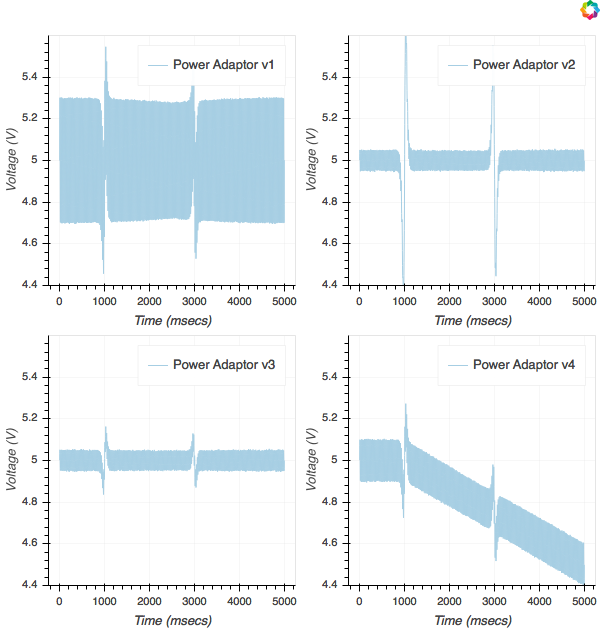
\includegraphics[width=\columnwidth]{imgs/powers}
	\label{fig:datos}
	\caption{Datos para las Fuentes de alimentacion V1, V2, V3 y V4.}
\end{figure}

En primer lugar, se analizar� cada fuente de forma individual. La primera fuente de alimentaci�n es la V1, cuyos valores est�n representados en la gr�fica de la parte superior izquierda. Se observa que la variaci�n en voltaje es amplia y casi mitiga las fases de carga-descarga. Este comportamiento tan oscilante no es adecuado para los dispositivos, as� que pasaremos a evaluar las otras alternativas. 

Para descartar otra fuente adicional, se considera la gr�fica que representa los valores de la fuente V4, en la parte inferior derecha. Esta fuente pierde la carga conforme pasa el tiempo, comportamiento no adecuado y por lo tanto se desestima su usa.

En cuanto a las fuentes V3 y V4, los valores sobre los que oscila el voltaje son aceptables en ambos casos, sin embargo, la fuente n�mero 2 presenta unos picos de carga/descarga demasiado elevados como para no suponer un riesgo para el equipo electr�nico conectado.

\section{Conclusi�n}

Concluyendo, se ha podido apreciar claramente c�mo la fuente de alimentaci�n m�s estable ser�a la fuente V3, dado que contiene una variabilidad de voltaje menor evidente, as� como unos picos de carga-descarga menos pronunciados.



\end{document}
